%%%%%%%%%%%%%%%%%%%%%%%%%%%%%%%%%%%%%%%%%%%%%%%%%%%%%%%%%%%%%%%%%%%%%%%%%
%  Zawartość: Główny plik szablonu pracy dyplomowej (magisterskiej/inżynierskiej).
%  Opracował: Tomasz Kubik <tomasz.kubik@pwr.edu.pl>
%  Data: kwiecień 2016
%  Wersja: 0.2
%%%%%%%%%%%%%%%%%%%%%%%%%%%%%%%%%%%%%%%%%%%%%%%%%%%%%%%%%%%%%%%%%%%%%%%%%

\documentclass[a4paper,onecolumn,oneside,12pt,extrafontsizes]{memoir}

% W celu przygotowania wydruku do archiwum należy przesłonić komendę powyższą
% dwoma poniższymi komendami:
%\documentclass[a4paper,onecolumn,twoside,10pt]{memoir} 
%\renewcommand{\normalsize}{\fontsize{8pt}{10pt}\selectfont}

%\usepackage[cp1250]{inputenc} % jeśli kodowanie edytowanych plików to cp1250 
\usepackage[utf8]{inputenc} % jeśli kodowanie edytowanych plików to UTF8
\usepackage[T1]{fontenc}
\usepackage[polish]{babel}
\usepackage{float}
%\DisemulatePackage{setspace}
\usepackage{setspace}
\usepackage{tabularx}
\usepackage{color,calc}
\usepackage{gensymb}
\usepackage{booktabs}
%\usepackage{soul} % pakiet z komendami do podkreślania tekstu

\usepackage{ebgaramond} % pakiet z czcionkami garamond, potrzebny tylko do strony tytułowej, musi wystąpić przed pakietem tgtermes

%% Aby uzyskać polskie literki w pdfie (a nie zlepki) korzystamy z pakietu czcionek tgterms. 
%% W pakiecie tym są zdefiniowane klony czcionek Times o kształtach: normalny, pogrubiony, italic, italic pogrubiony.
%% W pakiecie tym brakuje czcionki o kształcie: slanted (podobny do italic). 
%% Jeśli w dokumencie gdzieś zostanie zastosowana czcionka slanted (np. po użyciu komendy \textsl{}), to
%% latex dokona podstawienia na czcionkę standardową i zgłosi to w ostrzeżeniu (warningu).
%% Ponadto tgtermes to czcionka do tekstu. Wszelkie matematyczne wzory będą sformatowane domyślną czcionką do wzorów.
%% Jeśli wzory mają być sformatowane z wykorzystaniem innych czcionek, trzeba to jawnie zadeklarować.

%% Po zainstalowaniu pakietu tgtermes może będzie trzeba zauktualizować informacje 
%% o dostępnych fontach oraz mapy. Można to zrobić z konsoli (jako administrator)
%% initexmf --admin --update-fndb
%% initexmf --admin --mkmaps

\usepackage{tgtermes}   
\renewcommand*\ttdefault{txtt}

% We wcześniejszej wersji szablonu korzystano z innych czcionek. Dla celów historycznych pozostawiono je w komentarzu
%\usepackage{mathptmx} % pakiet będący następcą pakietów times and mathptm, niestety polskie literki są zlepkami
%\usepackage{newtxtext,newtxmath} % pakiety dostarczające Times dla tekstów i wzorów matematycznych,  
%                                  rozwiązuje problemy występujące w mathptmx, ale wymaga zainstalowania
%                                  dodatkowych pakietów oraz uruchomienia updmap (konsola administratora)
%                                  niestety polskie literki są zlepkami
%\usepackage{newtxmath,tgtermes} % można też połączyć czcionki do tekstu i czcionki do wzorów

\usepackage{listings} % pakiet do prezentacji kodu. 
%Wcześniej był problem z polskimi znakami w otoczeniu lstlisting, stąd pozostawiono w komentarzu zastosowane wtedy rozwiązanie: 
\lstset{literate=%-
{ą}{{\k{a}}}1 {ć}{{\'c}}1 {ę}{{\k{e}}}1 {ł}{{\l{}}}1 {ń}{{\'n}}1 {ó}{{\'o}}1 {ś}{{\'s}}1 {ż}{{\.z}}1 {ź}{{\'z}}1 {Ą}{{\k{A}}}1 {Ć}{{\'C}}1 {Ę}{{\k{E}}}1 {Ł}{{\L{}}}1 {Ń}{{\'N}}1 {Ó}{{\'O}}1 {Ś}{{\'S}}1 {Ż}{{\.Z}}1 {Ź}{{\'Z}}1 }%{\ \ }{{\ }}1}

% Choć możliwe jest zastosowanie różnych pakietów formatujących tabele, zaleca się tego nie robić.
%\usepackage{longtable}
%\usepackage{ltxtable}
%\usepackage{tabulary}

%%%%%%%%%%%%%%%%%%%%%%%%%%%%%%%%%%%%%%%%%%%%%%%%%%%
%% Ustawienia odpowiedzialne za sposób łamania dokumentu
%% i ułożenie elementów pływających
%%%%%%%%%%%%%%%%%%%%%%%%%%%%%%%%%%%%%%%%%%%%%%%%%%%
%\hyphenpenalty=10000		% nie dziel wyrazów zbyt często
\clubpenalty=10000      %kara za sierotki
\widowpenalty=10000  % nie pozostawiaj wdów
\brokenpenalty=10000		% nie dziel wyrazów między stronami
\exhyphenpenalty=999999		% nie dziel słów z myślnikiem
\righthyphenmin=3			% dziel minimum 3 litery

%\tolerance=4500
%\pretolerance=250
%\hfuzz=1.5pt
%\hbadness=1450

\renewcommand{\topfraction}{0.95}
\renewcommand{\bottomfraction}{0.95}
\renewcommand{\textfraction}{0.05}
\renewcommand{\floatpagefraction}{0.35}

%%%%%%%%%%%%%%%%%%%%%%%%%%%%%%%%%%%%%%%%%%%%%%%%%%%
%%  Ustawienia rozmiarów: tekstu, nagłówka i stopki, marginesów
%%  dla dokumentów klasy memoir 
%%%%%%%%%%%%%%%%%%%%%%%%%%%%%%%%%%%%%%%%%%%%%%%%%%%
\setlength{\headsep}{10pt} 
\setlength{\headheight}{13.6pt} % wartość baselineskip dla czcionki 11pt tj. \small wynosi 13.6pt
\setlength{\footskip}{\headsep+\headheight}
\setlength{\uppermargin}{\headheight+\headsep+1cm}
\setlength{\textheight}{\paperheight-\uppermargin-\footskip-1.5cm}
\setlength{\textwidth}{\paperwidth-5cm}
\setlength{\spinemargin}{2.5cm}
\setlength{\foremargin}{2.5cm}
\setlength{\marginparsep}{2mm}
\setlength{\marginparwidth}{2.3mm}
%\settrimmedsize{297mm}{210mm}{*}
%\settrims{0mm}{0mm}	
\checkandfixthelayout[fixed] % konieczne, aby się dobrze wszystko poustawiało
%%%%%%%%%%%%%%%%%%%%%%%%%%%%%%%%%%%%%%%%%%%%%%%%
%%  Ustawienia odległości linii, wcięć, odstępów
%%%%%%%%%%%%%%%%%%%%%%%%%%%%%%%%%%%%%%%%%%%%%%%%
\linespread{1}
%\linespread{1.241}
\setlength{\parindent}{14.5pt}
%\setbeforesecskip{10pt plus 0.5ex}%{-3.5ex \@plus -1ex \@minus -.2ex}
%\setaftersecskip{10pt plus 0.5ex}%\onelineskip}
%\setbeforesubsecskip{8pt plus 0.5ex}%{-3.5ex \@plus -1ex \@minus -.2ex}
%\setaftersubsecskip{8pt plus 0.5ex}%\onelineskip}
%\setlength\floatsep{6pt plus 2pt minus 2pt} 
%\setlength\intextsep{12pt plus 2pt minus 2pt} 
%\setlength\textfloatsep{12pt plus 2pt minus 2pt} 

%%%%%%%%%%%%%%%%%%%%%%%%%%%%%%%%%%%%%%%%%%%%%%%%%%%
%%  Pakiety i komendy zastosowane tylko do zamieszczenia informacji o użytych komendach i fontach
%%  Normalnie nie są potrzebne, można je zamarkować podczas redakcji pracy
%%%%%%%%%%%%%%%%%%%%%%%%%%%%%%%%%%%%%%%%%%%%%%%%%%%
\usepackage{memlays}     % extra layout diagrams, zastosowane w szblonie do 'debuggowania', używa pakietu layouts
%\usepackage{layouts}
\usepackage{printlen} % pakiet do wyświetlania wartości zdefiniowanych długości, stosowany do 'debuggowania'
\uselengthunit{pt}
\makeatletter
\newcommand{\showFontSize}{\f@size pt} % makro wypisujące wielkość bieżącej czcionki
\makeatother
% do pokazania ramek można byłoby użyć:
%\usepackage{showframe} 


%%%%%%%%%%%%%%%%%%%%%%%%%%%%%%%%%%%%%%%%%%%%%%%%%%%
%%  Formatowanie list wyliczeniowych, wypunktowań i własnych otoczeń
%%%%%%%%%%%%%%%%%%%%%%%%%%%%%%%%%%%%%%%%%%%%%%%%%%%

% Domyślnie wypunktowania mają zadeklatorowane znaki, które nie występują w tgtermes
% Aby latex nie podstawiał w ich miejsca znaków z czcionki standardowej można zrobić podstawienie:
%    \DeclareTextCommandDefault{\textbullet}{\ensuremath{\bullet}}
%    \DeclareTextCommandDefault{\textasteriskcentered}{\ensuremath{\ast}}
%    \DeclareTextCommandDefault{\textperiodcentered}{\ensuremath{\cdot}}
% Jednak jeszcze lepszym pomysłem jest zdefiniowanie otoczeń z wykorzystaniem enumitem
\usepackage{enumitem} % pakiet pozwalający zarządzać formatowaniem list wyliczeniowych
\setlist{noitemsep,topsep=4pt,parsep=0pt,partopsep=4pt,leftmargin=*} % zadeklarowane parametry pozwalają uzyskać 'zwartą' postać wypunktowania bądź wyliczenia
\setenumerate{labelindent=0pt,itemindent=0pt,leftmargin=!,label=\arabic*.} % można zmienić \arabic na \alph, jeśli wyliczenia mają być z literkami
\setlistdepth{4} % definiujemy głębokość zagnieżdżenia list wyliczeniowych do 4 poziomów
\setlist[itemize,1]{label=$\bullet$}  % definiujemy, jaki symbol ma być użyty w wyliczeniu na danym poziomie
\setlist[itemize,2]{label=\normalfont\bfseries\textendash}
\setlist[itemize,3]{label=$\ast$}
\setlist[itemize,4]{label=$\cdot$}
\renewlist{itemize}{itemize}{4}

%%%http://tex.stackexchange.com/questions/29322/how-to-make-enumerate-items-align-at-left-margin
%\renewenvironment{enumerate}
%{
%\begin{list}{\arabic{enumi}.}
%{
%\usecounter{enumi}
%%\setlength{\itemindent}{0pt}
%%\setlength{\leftmargin}{1.8em}%{2zw} % 
%%\setlength{\rightmargin}{0zw} %
%%\setlength{\labelsep}{1zw} %
%%\setlength{\labelwidth}{3zw} % 
%\setlength{\topsep}{6pt}%
%\setlength{\partopsep}{0pt}%
%\setlength{\parskip}{0pt}%
%\setlength{\parsep}{0em} % 
%\setlength{\itemsep}{0em} % 
%%\setlength{\listparindent}{1zw} % 
%}
%}{
%\end{list}
%}
\makeatletter
\renewenvironment{quote}{
	\begin{list}{}
	{
	\setlength{\leftmargin}{1em}
	\setlength{\topsep}{0pt}%
	\setlength{\partopsep}{0pt}%
	\setlength{\parskip}{0pt}%
	\setlength{\parsep}{0pt}%
	\setlength{\itemsep}{0pt}
	}
	}{
	\end{list}}
\makeatother

%%%%%%%%%%%%%%%%%%%%%%%%%%%%%%%%%%%%%%%%%
%%  Pakiet do generowania indeksu (ważne, aby wstawić przed hyperref)
%%%%%%%%%%%%%%%%%%%%%%%%%%%%%%%%%%%%%%%%%
\DisemulatePackage{imakeidx}
\usepackage[makeindex,noautomatic]{imakeidx} % tutaj mówimy, żeby indeks nie generował się automatycznie, 

%\usepackage[noautomatic]{imakeidx} 
\makeindex

\makeatletter
%%%\renewenvironment{theindex}
							 %%%{\vskip 10pt\@makeschapterhead{\indexname}\vskip -3pt%
								%%%\@mkboth{\MakeUppercase\indexname}%
												%%%{\MakeUppercase\indexname}%
								%%%\vspace{-3.2mm}\parindent\z@%
								%%%\renewcommand\subitem{\par\hangindent 16\p@ \hspace*{0\p@}}%%
								%%%\phantomsection%
								%%%\begin{multicols}{2}
								%%%%\thispagestyle{plain}
								%%%\parindent\z@                
								%%%%\parskip\z@ \@plus .3\p@\relax
								%%%\let\item\@idxitem}
							 %%%{\end{multicols}\clearpage}
%%%
\makeatother


\usepackage{ifpdf}
%\newif\ifpdf \ifx\pdfoutput\undefined
%\pdffalse % we are not running PDFLaTeX
%\else
%\pdfoutput=1 % we are running PDFLaTeX
%\pdftrue \fi
\ifpdf
 \usepackage[pdftex,bookmarks,breaklinks,unicode]{hyperref}
 \usepackage[pdftex]{graphicx}
 \DeclareGraphicsExtensions{.pdf,.jpg,.mps,.png}
\pdfcompresslevel=9
\pdfoutput=1
\makeatletter
\AtBeginDocument{
  \hypersetup{
	pdfinfo={
    Title = {\@title},
    Author = {\@author},
    Subject={},
    Keywords={słowa kluczowe},
  }}
}
\makeatother
\else
\usepackage{graphicx}
\DeclareGraphicsExtensions{.eps,.ps,.jpg,.mps,.png}
\fi
\sloppy


%\graphicspath{{rys01/}{rys02/}}


%%%%%%%%%%%%%%%%%%%%%%%%%%%%%%%%%%%%%%%%%
% Metadane dla pdfa


%\ifpdf
%\pdfinfo{
   %/Author (Nicola Talbot)
   %/Title  (Creating a PDF document using PDFLaTeX)
   %/CreationDate (D:20040502195600)
   %/ModDate (D:\pdfdate)
   %/Subject (PDFLaTeX)
   %/Keywords (PDF;LaTeX)
%}
%\fi

% Deklaracja głębokościu numeracji
\setcounter{secnumdepth}{2}
\setcounter{tocdepth}{2}
\setsecnumdepth{subsection} % activating subsubsec numbering in doc


% Kropki po numerach sekcji
\makeatletter
\def\@seccntformat#1{\csname the#1\endcsname.\quad}
\def\numberline#1{\hb@xt@\@tempdima{#1\if&#1&\else.\fi\hfil}}
\makeatother

\renewcommand{\chapternumberline}[1]{#1.\quad}
\renewcommand{\cftchapterdotsep}{\cftdotsep}

%\definecolor{niceblue}{rgb}{.168,.234,.671}

% Czcionka do podpisów tabel i rysunków
\captionnamefont{\small}
\captiontitlefont{\small}
% makro pozwalające zmienić sposób wypisywania rozdziału
%\def\printchaptertitle##1{\fonttitle \space \thechapter.\space ##1} 

%\usepackage{ltcaption}
% The ltcaption package supports \CaptionLabelFont & \CaptionTextFont introduced by the NTG document classes
%\renewcommand\CaptionLabelFont{\small}
%\renewcommand\CaptionTextFont{\small}

% Przedefiniowanie etykiet w podpisach tabel i rysunków
%\AtBeginDocument{% 
        \addto\captionspolish{% 
        \renewcommand{\tablename}{Tab.}% 
}%} 

%\AtBeginDocument{% 
%        \addto\captionspolish{% 
%        \renewcommand{\chaptername}{Rozdział}% 
%}} 

%\AtBeginDocument{% 
        \addto\captionspolish{% 
        \renewcommand{\figurename}{Rys.}% 
}%}


%\AtBeginDocument{% 
        \addto\captionspolish{% 
        \renewcommand{\bibname}{Literatura}% 
}%}

%\AtBeginDocument{% 
        \addto\captionspolish{% 
        \renewcommand{\listfigurename}{Spis rysunków}% 
}%}

%\AtBeginDocument{% 
        \addto\captionspolish{% 
        \renewcommand{\listtablename}{Spis tabel}% 
}%}

%\AtBeginDocument{% 
        \addto\captionspolish

%%%%%%%%%%%%%%%%%%%%%%%%%%%%%%%%%%%%%%%%%%%%%%%%%%%%%%%%%%%%%%%%%%                  
%% Definicje stopek i nagłówków
%%%%%%%%%%%%%%%%%%%%%%%%%%%%%%%%%%%%%%%%%%%%%%%%%%%%%%%%%%%%%%%%%%                  
\addtopsmarks{headings}{%
\nouppercaseheads % added at the beginning
}{%
\createmark{chapter}{both}{shownumber}{}{. \space}
%\createmark{chapter}{left}{shownumber}{}{. \space}
\createmark{section}{right}{shownumber}{}{. \space}
}%use the new settings

\makeatletter
\copypagestyle{outer}{headings}
\makeoddhead{outer}{}{}{\small\itshape\rightmark}
\makeevenhead{outer}{\small\itshape\leftmark}{}{}
\makeoddfoot{outer}{\small\@author:~\@titleShort}{}{\small\thepage}
\makeevenfoot{outer}{\small\thepage}{}{\small\@author:~\@title}
\makeheadrule{outer}{\linewidth}{\normalrulethickness}
\makefootrule{outer}{\linewidth}{\normalrulethickness}{2pt}
\makeatother

% fix plain
\copypagestyle{plain}{headings} % overwrite plain with outer
\makeoddhead{plain}{}{}{} % remove right header
\makeevenhead{plain}{}{}{} % remove left header
\makeevenfoot{plain}{}{}{}
\makeoddfoot{plain}{}{}{}

\copypagestyle{empty}{headings} % overwrite plain with outer
\makeoddhead{empty}{}{}{} % remove right header
\makeevenhead{empty}{}{}{} % remove left header
\makeevenfoot{empty}{}{}{}
\makeoddfoot{empty}{}{}{}


%%%%%%%%%%%%%%%%%%%%%%%%%%%%%%%%%%%%%%%
%% Definicja strony tytułowej 
%%%%%%%%%%%%%%%%%%%%%%%%%%%%%%%%%%%%%%%
\makeatletter
%Uczelnia
\newcommand\uczelnia[1]{\renewcommand\@uczelnia{#1}}
\newcommand\@uczelnia{}
%Wydział
\newcommand\wydzial[1]{\renewcommand\@wydzial{#1}}
\newcommand\@wydzial{}
%Kierunek
\newcommand\kierunek[1]{\renewcommand\@kierunek{#1}}
\newcommand\@kierunek{}
%Specjalność
\newcommand\specjalnosc[1]{\renewcommand\@specjalnosc{#1}}
\newcommand\@specjalnosc{}
%Tytuł po angielsku
\newcommand\titleEN[1]{\renewcommand\@titleEN{#1}}
\newcommand\@titleEN{}
%Tytuł krótki
\newcommand\titleShort[1]{\renewcommand\@titleShort{#1}}
\newcommand\@titleShort{}
%Promotor
\newcommand\promotor[1]{\renewcommand\@promotor{#1}}
\newcommand\@promotor{}

%\usepackage[absolute]{textpos} % zamarkowano, bo ostatecznie wykorzystano otoczenie picture

\def\maketitle{%
  \pagestyle{empty}%
% \garamond 
	\fontfamily{\ebgaramond@family}\selectfont % na stronie tytułowej czcionka garamond
%%%%%%%%%%%%%%%%%%%%%%%%%%%%%%%%%%%%%	
%% Poniżej, w otoczniu picture, wstawiono tytuł i autora. 
%% Tytuł (z autorem) musi znaleźć się w obszarze 
%% odpowiadającym okienku 110mmx75mm, którego lewy górny róg 
%% jest w położeniu 77mm od lewej i 111mm od górnej  krawędzi strony 
%% (tak wynika z wycięcia na okładce). 
%% Poniższy kod musi być użyty dokładnie w miejscu gdzie jest.
%% Jeśli tytuł nie mieści się w okienku, to należy tak pozmieniać 
%% parametry użytych komend, aby ten przydługi tytuł jednak 
%% upakować go do okienka.
%%
%% Sama okładka (kolorowa strona z wycięciem, do pobrania z dydaktyki) 
%% powinna być przycięta o 3mm od każdej z krawędzi.
%% Te 3mm pewnie zostawiono na ewentualne spady czy też specjalną oprawę.
%%%%%%%%%%%%%%%%%%%%%%%%%%%%%%%%%%%%%	
\newlength{\tmpfboxrule}
\setlength{\tmpfboxrule}{\fboxrule}
\setlength{\fboxsep}{2mm}
\setlength{\fboxrule}{0mm} 
%\setlength{\fboxrule}{0.1mm} %% jeśli chcemy zobaczyć ramkę
\setlength{\unitlength}{1mm}
\begin{picture}(0,0)
\put(26,-124){\fbox{
\parbox[c][71mm][c]{104mm}{\centering%\lineskip=34pt 
\fontsize{16pt}{18pt}\selectfont \@title\\[5mm]
\fontsize{16pt}{18pt}\selectfont \@titleEN\\[20mm]
\fontsize{16pt}{18pt}\selectfont AUTOR:\\[2mm]
\fontsize{14pt}{16pt}\selectfont \@author}
}
}
\end{picture}
\setlength{\fboxrule}{\tmpfboxrule} 
%%%%%%%%%%%%%%%%%%%%%%%%%%%%%%%%%%%%%
%% Reszta strony z nazwą uczelni, wydziału, kierunkiem, specjalnością
%% promotorem, oceną pracy, miastem i rokiem
	{\centering%\vspace{-1cm}
		{\fontsize{22pt}{24pt}\selectfont \@uczelnia}\\[0.4cm]
		{\fontsize{22pt}{24pt}\selectfont \@wydzial}\\[0.5cm]
		  \hrule %\vspace*{0.7cm}
	}
{\flushleft\fontsize{14pt}{16pt}\selectfont%
\begin{tabular}{ll}
KIERUNEK: & \@kierunek\\
SPECJALNOŚĆ: & \@specjalnosc\\
\end{tabular}\\[1.3cm]
}
{\centering
{\fontsize{32pt}{36pt}\selectfont PRACA DYPLOMOWA}\\[0.5cm]
{\fontsize{32pt}{36pt}\selectfont MAGISTERSKA}\\[2.5cm]
}
\vfill
\begin{tabularx}{\linewidth}{p{6cm}l}
		&{\fontsize{16pt}{18pt}\selectfont PROWADZĄCY PRACĘ:}\\[2mm] %UWAGA: tutaj jest miejsce na nazwisko promotora pracy
		&{\fontsize{14pt}{16pt}\selectfont \@promotor}\\[10mm]
		&{\fontsize{16pt}{18pt}\selectfont OCENA PRACY:}\\[20mm]
	\end{tabularx}
\vspace{2cm}
\hrule\vspace*{0.3cm}
{\centering
{\fontsize{16pt}{18pt}\selectfont \@date}\\[0cm]
}
%\ungaramond
\normalfont
 \cleardoublepage
}
\makeatother
%%%%%%%%%%%%%%%%%%%%%%%%%%%%%%%%%%%%%%%%%

\AtBeginDocument{\addtocontents{toc}{\protect\thispagestyle{empty}}}




%%%%%%%%%%%%%%%%%%%%%%%%%%%%%%%%%%%%%%%%%
%%  Metadane dokumentu 
%%%%%%%%%%%%%%%%%%%%%%%%%%%%%%%%%%%%%%%%%
\title{Zastosowanie metod uczenia maszynowego w detekcji fałszywych informacji}
\titleShort{Zastosowanie metod uczenia maszynowego w detekcji fałszywych informacji}
\titleEN{Application of machine learning methods to fake news detection}
\author{Inż. Dawid Mikowski}
\uczelnia{POLITECHNIKA WROCŁAWSKA}
\wydzial{WYDZIAŁ ELEKTRONIKI}
\kierunek{INFORMATYKA}
\specjalnosc{Inżynieria systemów informatycznych}
\promotor{Prof. Michał Woźniak}
\date{WROCŁAW, 2020}

% Ustawienie odstępu od góry w nienumerowanych rozdziałach oraz wykazach:
% Spis treści, Spis tabel, Spis rysunków, Indeks rzeczowy

%\newlength{\linespace}
%\setlength{\linespace}{-\beforechapskip-\topskip+\headheight+\topsep}
%\makechapterstyle{noNumbered}{%
%\renewcommand\chapterheadstart{\vspace*{\linespace}}
%}

%% powyższa komenda załatwia to, co robią komendy poniższe dla spisów
%\renewcommand*{\tocheadstart}{\vspace*{\linespace}}
%\renewcommand*{\lotheadstart}{\vspace*{\linespace}}
%\renewcommand*{\lofheadstart}{\vspace*{\linespace}}

%%%%%%%%%%%%%%%%%%%%%%%%%%%%%%%%%%%%%%%%%
%                  Początek dokumentu 
%%%%%%%%%%%%%%%%%%%%%%%%%%%%%%%%%%%%%%%%%
%\includeonly{skroty,rozdzial01} % jeśli chcemy kompilować tylko fragmenty, to można tu je wpisać

\begin{document}
% Tutaj można przełączyć odstęp między liniami
%\SingleSpacing
%\OnehalfSpacing
%\DoubleSpacing

%\settypeoutlayoutunit{cm} % do debugowania
%\typeoutstandardlayout    % wypisuje na stdout informacje o ustawieniach
\maketitle

\chapterstyle{noNumbered}
\pagestyle{outer}
\mbox{}\pdfbookmark[0]{Spis treści}{spisTresci.1}
\tableofcontents* 

\newpage
% \mbox{}\pdfbookmark[0]{Spis rysunków}{spisRysunkow.1}
% \addcontentsline{toc}{chapter}{Spis rysunków}
% \listoffigures*
{%
\let\oldnumberline\numberline%
\renewcommand{\numberline}{\figurename~\oldnumberline}%
\listoffigures%
}
\newpage


% \newpage
% \mbox{}\pdfbookmark[0]{Spis tabel}{spisTabel.1}
% \addcontentsline{toc}{chapter}{Spis tabel}
% \listoftables*

% \chapter*{Skróty}\mbox{}\pdfbookmark[0]{Skróty}{skroty.1}
\label{sec:skroty}
\noindent
\begin{description}
  \item [CRC] Rodzaj sumy kontrolnej (ang.\ \emph{Cyclic Redundancy Check})
  
\end{description}
 %skróty można sobie pominąć
\chapterstyle{default}
\chapter*{Wstęp}
\section*{Motywacja}
Ogromna w ostatnich latach popularność różnego rodzaju mediów społecznościowych, a co za tym 
idzie wymiany ogromnej ilości informacji między ludźmi powoduje, że tak jak nigdy wcześniej 
w historii spotkać się można z masową dezinformacją i skutkami jakie może ona ze sobą nieść.
Nieprawdziwe informacje stanowią realne zagrożenie dla każdego z nas dlatego odnalezienie 
prostego sposobu na ich wykrycie staje się coraz ważniejsze i mogłoby pozwolić na 
zredukowanie lub całkowite wyeliminowanie szansy na bycie oszukanym podczas zbierania
informacji z różnych stron internetowych. Popularne ostatnimi czasy algorytmy uczenia 
maszynowego mogą stanowić rozwiązanie tego problemu.
\section*{Cel pracy}
Celem pracy jest sprawdzenie efektywności popularnych algorytmów uczenia maszynowego w rozwiązywaniu 
zadania klasyfikacji tekstów na prawdziwe i nieprawdziwe informacje. Badana metoda opiera 
się na analizie tekstu podzielonego na tak zwane NGramy czyli sekwencje jednego lub kilku znaków.
Metoda ta jest stosowana podczas detekcji spamu w różnego rodzaju skrzynkach mailowych.
W badaniu sprawdzano jak zmiana długości NGramów wpływa na efektywność algorytmów czas ich 
uczenia oraz czas wykonywania przez nie predykcji. 
\section*{Zawartość pracy}
Praca składa się z sześciu rodziałów pierwsze trzy zawierają teoretyczne wprowadzenie 
do tematów związanych z celem pracy. Kolejne dwa rozdziały składają się z opisu metod jakie 
zostały wykorzystane do osiągnięcia celu oraz analizę wykonanych badań. Ostatni rozdział 
stanowi podsumowanie całej pracy.

Dokładny opis zawartości każdego z rozdziałów wygląda następująco:
\begin{enumerate}
    \item W pierwszym rozdziale krótko została opisana historia nieprawdziwych informacji 
    i ich rozprzestrzeniania. Zdefiniowano pojęcie fake news i omówiono jego znaczenie w
    dzisiejszym świecie. Omówiono także sposoby ochrony przed nieprawdziwymi informacjami.
    Opisano także zagrożenie jakie stanowi stworzona w ostatnich latach technologia o 
    nazwie deepfake.
    \item Rozdział drugi zawiera opis technologii jaką jest uczenie maszynowe. Zostały
    omówione jedne z popularniejszych algorytmów uczenia maszynowego, które wykorzystano
    do wykonania badań. Został także uwzględniony opis zagrożenia jakie może stanowić uczenie
    maszynowe dla ludzkości.
    \item Trzeci rozdział krótko opisuje dziedzinę informatyki, którą jest przetwarzanie 
    języków naturalnych. Zostały opisane przykłady jej zastosowania w dzisiejszym świecie.
    Krótko omówione zostały także sposoby przygotowywania danych tekstowych. Ostatnim elementem
    rozdziału jest opis metod wektoryzacji czyli zamiany tekstu na formę numeryczną. 
    \item W rozdziale czwartym zawarty jest opis systemu, który został 
    stworzony w celu wykonania badań. Opisano wykorzystane w nim technologie oraz motywację 
    wyboru każdego z nich. Wymieniono wymagania funkcjonalne, które musi spełniać ten system oraz
    zawarto krótki opis jego implementacji.
    \item Piąty rozdział zawiera ocenę eksperymentalną wykonanych badań. Opisane są w nim 
    warunki przeprowadzonego eksperymentu wraz ze specyfikacją danych, wyniki badań a także 
    analiza wyników. Na zakończenie rozdziału sformułowano wnioski wynikające z wyników badań.  
\end{enumerate}
\chapter{Informacje nieprawdziwe w dobie internetu}
Pojęcie ``Fake news'' odnosi się do 
informacji, które pomimo że nie posiadają pokrycia z rzeczywistością są 
przedstawiane jako prawdziwe w mediach takich jak np.: wiadomości, artykuły, 
portale społecznościowe itd.. 
Zwrot ten jest neologizmem i w języku angielskim oznacza dosłownie ``Fałszywe wiadomości''
celem wykorzystania takich wiadomości mogą być żarty np.: satyra, jednak najczęsciej 
mają one za zadanie oszukać odbiorce i wpłynąć na jego poglądy w sposób żądany przez autora
danej informacji. 

Fake news'y stały się bardzo popularnym zagadnieniem w ostatnich czasach ponieważ
internet a w szczególności media społecznościowe pozwoliły na przekazywanie 
informacji z niespotykaną wcześniej prędkością dzięki czemu rozprzestrzenianie 
dezinformacji stało się zadaniem stosunkowo prostym.

Zagadnienie to zyskało ogromny rozgłos podczas kampanii wyborczej oraz
prezydentury Donalda Trumpa, który zasłynął z częstego wykorzystywania 
tego zwrotu podczas wywiadów debat oraz wypowiedzi na mediach społecznościowych
tj. Twitter.
Do roku 2020 pojęcie ``Fake News'' zostało umieszczone w słownikach języka angielskiego
takich jak ``Oxford English Dictionary'', ``Macmillan Dictionary''.
\begin{figure}[h!]
    \centering
    
\includegraphics[width=0.7\textwidth]{./Img/Trump-Fake-News.png}
    \caption{Post udostępniony przez Donalda Trumpa na portalu Twitter}
\end{figure}

Według założonego przez dziewięć organizacji w skład których wchodzą 
Google, Facebook oraz Twitter projektu ``First Draft News''
możemy wyróżnić siedem typów Fake Newsów.
\begin{enumerate}
    \item Satyra bądź parodia
    \item Fałszywe połączenie
    \item Myląca zawartość
    \item Fałszywy kontekst
    \item Oszukana zawartość
    \item Zmanipulowana zawartość
    \item Sfabrykowana zawartość
\end{enumerate}
\section{Sposoby rozprzestrzeniania fałszywych informacji}

\section{Deep fake}

\section{Sposoby ochrony przed nieprawdziwymi informacjami}

\chapter{Uczenie maszyn}
Uczenie maszynowe jest dziedziną algorytmów komputerowych, które automatycznie poprawiają swoją poprawność poprzez doświadczenie. 
Określa się je jako poddziedzinę sztucznej inteligencji. Algorytmy te pozwalają na zbudowanie matematycznego modelu na podstawie 
przykładowych danych nazywanych danymi treningowymi, co pozwala im na wykonywanie predykcji lub decyzji bez potrzeby ich dokładnego 
zaimplementowania przez programistę. 


Uczenie maszynowe stosuje się do wielu zadań, między innymi do filtrowania poczty mailowej ze spamu, reklam internetowych, 
wykrywania twarzy na zdjęciach oraz nagraniach, a w przyszłości może pomóc w stworzeniu technologii takich jak 
autonomiczne samochody. Sam termin został spopularyzowany przez informatyka Arhura Samuela w roku 1959, który był autorem pierwszego działającego 
systemu tego typu. Jego program automatycznie grał w warcaby i uczył się na podstawie poprzednich potyczek ~\cite{MLBasics}. 


W dzisiejszych czasach implementacja takich systemów opiera się na wykonaniu następujących czynności:
\begin{itemize}
    \item preprocessing danych:
    \begin{itemize}
        \item czyszczenie,
        \item uzupełnianie,
        \item redukcja wymiarowości.
    \end{itemize}
    \item ekstrakcja cech,
    \item uczenie modelu,
    \item sprawdzenie poprawności modelu.
\end{itemize}
Odpowiednie wykonanie etapu ekstrakcji cech jest kluczowym elementem do stworzenia poprawnego modelu, jest
on opisany w kolejnym rozdziale pracy. 



Ogromny rozwój uczenia maszynowego i sztucznej inteligencji spowodował, że znalazły one 
wiele zastosowań w różnych dziedzinach życia codziennego. Powoduje to, że wiele osób skupia się 
na pozytywach związanych
z tymi technologiami, jednakże niektórzy dostrzegają ogromne zagrożenia płynące z niewłaściwego 
wykorzystania ich i katastrofalne skutki, do których mogą doprowadzić. 
Wśród takich osób znajdują się naukowcy tacy jak Stephen Hawking, Elon Musk, Steve Wozniak i Bill Gates. 
Według Elona Muska sztuczna inteligencja niesie ze sobą większe zagrożenie niż bomby atomowe ~\cite{dangers}. 

Dwa główne sposoby w jaki sztuczna inteligencja może powodować zagrożenie to:
\begin{itemize}
    \item AI zaprogramowane do czynienia krzywdy, czyli na przykład wykorzystanie uczenia maszynowego
    w takich narzędziach jak broń, która w niewłaściwych rękach stanowiłaby zagrożenie dla całej ludzkości,
    \item AI zaprogramowane w dobrych celach, jednak odnajdujące krzywdzący innych optymalny
    sposób osiągnięcia sukcesu, może to być związane ze złym przekazaniem celu jaki maszyna ma osiągnąć, przez 
    programistę. Przykładowo, mógłby to być samojezdny samochód, który podczas jazdy zwraca uwagę tylko i wyłącznie 
    na to by jak najszybciej dojechać do celu podróży. Samochód taki nie przestrzegałby istniejących praw drogowych,
    ponieważ ograniczałyby one jego prędkość.
\end{itemize}
Przykłady te pokazują, że zagrożenie nie płynie z sytuacji gdzie maszyny odwracają się przeciwko ludzkości, lecz 
z sytuacji, w której maszyny wykonują poświęcone im zadania za dobrze i nie w sposób przewidziany przez 
stwórcę systemu.

Istotnym problemem jest także bezrobocie będące skutkiem zastępowania ludzi maszynami,
ponieważ są one znacznie tańsze w utrzymaniu niż pracownicy, a z wykorzystaniem uczenia
maszynowego mogą one opanować niektóre zadania lepiej od ludzi.
Rozwiązaniem na takie problemy mogłyby być obowiązkowo przestrzegane zasady bezpiecznego korzystania
ze sztucznej inteligencji, których złamanie wiązałoby się z odpowiedzialnością karną.
\section{Rodzaje uczenia na podstawie przykładów}

Algorytmy uczenia maszynowego uczące się na podstawie przykładów można podzielić na dwa główne rodzaje w zależności od problemów, które mają one rozwiązywać:
\begin{itemize}
    \item uczenie nadzorowane -
    jest to najczęściej wykorzystywany rodzaj uczenia maszynowego, polega on na tym,
    że maszyna uczy się na podstawie przykładów zawartych w danych treningowych.
    Uczenie nadzorowane można porównać do nauczyciela i ucznia gdzie dane pełnią rolę nauczyciela, 
    a program ucznia. Algorytmy tego typu potrafią znaleźć odpowiednie zależności na podstawie
    etykiet przypisanym danym,
    które następnie wykorzystują w celu predykcji wcześniej nie analizowanych danych.
    Ważnym zagadnieniem w przypadku uczenia nadzorowanego jest tak zwany overfitting polegający 
    na przeuczeniu programu jednym zestawem treningowym, przez co traci on umiejętność generalizacji problemu
    i nie jest w stanie poprawnie podejmować predykcji danych niewystarczająco podobnych
    do treningowych.

    Przykładowe zastosowania:
    \begin{itemize}
        \item klasyfikacja - przewidywanie kategorii:
        \begin{itemize}
            \item rozpoznawanie elementów na zdjęciu,
            \item filtrowanie spamu w skrzynce mailowej.
        \end{itemize}
        \item regresja - przewidywanie liczb:
        \begin{itemize}
            \item przewidywanie trendów finansowych lub ekonomicznych,
            \item prognozowanie pogody.
        \end{itemize}
    \end{itemize}
    \item uczenie nienadzorowane -
    w przeciwieństwie do uczenia nadzorowanego, opiera się na braku
    nauczyciela, a zadaniem maszyny jest znalezienie wzorców i zależności między analizowanymi
    obiektami samodzielnie. Dwie metody które są najczęściej wykorzystywane w uczeniu nienadzorowanym
    to:
    \begin{itemize}
        \item analiza składowych głównych - polega na zmniejszaniu wymiarowości danych poprzez
        odnajdywanie, a następnie odrzucanie cech, które niosą ze sobą najmniejszą ilość informacji,
        \item analiza skupień (Klasteryzacja) - pozwala na identyfikację oraz grupowanie danych
        podobnych, które nie są w żaden sposób oznaczone. Może także pomóc w odnalezieniu anomalii
        nie pasujących do żadnej z wydzielonych grup.
        
    \end{itemize} 
    Wykorzystanie tego typu algorytmów pozwala na badanie danych nieoznaczonych,
    które są znacznie częściej spotykane niż dane oznaczone.
    
    Przykładowe zastosowania:
    \begin{itemize}
        \item redukcja wymiarów:
        \begin{itemize}
            \item wizualizacja danych ``big data'',
            \item kompresja danych.
        \end{itemize}
        \item klasteryzacja:
        \begin{itemize}
            \item spersonalizowane reklamy,
            \item systemy rekomendacyjne.
        \end{itemize}
    \end{itemize}
\end{itemize} 
\section{Algorytmy klasyfikacji}
Z problemem klasyfikacji można się spotkać wszędzie tam, gdzie wykorzystując
zbiór zmiennych objaśniających należy wskazać wartość przyjmowaną przez zmienną
modelowaną. W problemach klasyfikacji zmienna modelowana może przyjmować wartości
binarne (klasyfikacja dwuklasowa) lub jedną z wielu etykiet (klasyfikacja wieloklasowa).
Aby wybrać odpowiedni do rozwiązywanego problemu algorytm klasyfikacji należy wziąć 
pod uwagę cztery czynniki:
\begin{itemize}
    \item złożoność czasowa - jak długo trwa uczenie oraz predykcja nowych danych,
    \item interpretowalność - jak łatwo można wytłumaczyć decyzję podjętą przez 
    system,
    \item skalowalność - jak dużą ilość zasobów zużywa dany algorytm,
    \item czynnik ludzki - aby poprawnie ustawić parametry algorytmu potrzebna
    jest wiedza na temat jego działania, ponieważ poprawne ich ustawienie może 
    mieć większe znaczenie dla efektywności niż dobór najlepszego algorytmu. Często
    lepiej jest wykorzystać algorytm znany, a nie optymalny.
\end{itemize}
W dalszej części rodziału opisane zostały najpopularniejsze metody klasyfikacji.
\subsection{K najbliższych sąsiadów}

Algorytm K najbliższych sąsiadów (K nearest neighbours) jest algorytmem
stosowanym zarówno w problemach regresyjnych, jak i klasyfikacji. Kroki jego działania
można opisać w następujący sposób:
\begin{itemize}
    \item umieszczenie wszystkich obiektów posiadających N cech jako punkty w N-wymiarowej przestrzeni,
    \item obliczenie odległości między obiektem, którego etykieta będzie przewidywana, a każdym innym
    obiektem,
    \item przypisanie do obiektu etykiety, którą posiada większość z K najbliższych obiektów. 
\end{itemize}
Faza uczenia w \textit{k}-NN polega wyłącznie na wczytaniu danych treningowych do pamięci, przez co jest 
ona bardzo szybka.

Najważniejszą kwestią w poprawnym implementowaniu algorytmu \textit{k}-NN jest odpowiednie wybranie liczby
K, której optymalna wartość będzie się różnić w zależności od danych. W problemach 
klasyfikacji często wybiera się K o wartości nieparzystej aby uniknąć problemu remisu
podczas zliczania sąsiadów. W przypadku problemów regresyjnych zamiast wykonywać głosowanie,
predykcję wykonuje się na podstawie średniej wartości K najbliższych sąsiadów ~\cite{MLAlgorithms}.

\begin{table}[h]
    \begin{tabularx}{\linewidth}{>{\parskip1ex}X@{\kern4\tabcolsep}>{\parskip1ex}X}
    \toprule
    \hfil\bfseries Zalety
    &
    \hfil\bfseries Wady
    \\\cmidrule(r{3\tabcolsep}){1-1}\cmidrule(l{-\tabcolsep}){2-2}
    
    %% PROS, seperated by empty line or \par
    prosty do zrozumienia i interpretacji,\par
    szybkość fazy uczenia,\par
    nie wykonuje generalizacji danych, przez co jest efektywny w przypadku danych nieliniowych.\par
    &
    
    %% CONS, seperated by empty line or \par
    przechowuje wszystkie dane treningowe w pamięci, co skutkuje wysoką złożonością pamięciową,\par
    wrażliwy na ilość danych i nieistotne cechy,\par
    kosztowny obliczeniowo.\par
    \\\bottomrule
    \end{tabularx}
    \caption{Wady i zalety \textit{k}-NN}
\end{table}
    

\begin{figure}[H]
    \centering
    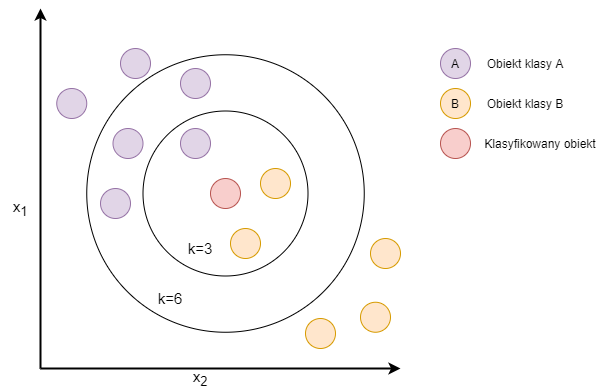
\includegraphics[width=0.8\textwidth]{./Img/KNN.png}
    \caption{Graficzne przedstawienie algorytmu \textit{k}-NN Źródło: Własne}
\end{figure}

\subsection{Maszyna wektorów nośnych}

Klasyfikator SVM (Support vector machines) można wykorzystywać zarówno 
w problemach regresyjnych i klasyfikacyjnych. Służą one do klasyfikacji binarnej, co 
oznacza, że obiekty należy podzielić na dokładnie dwie klasy. SVM polega na znalezieniu
takiej prostej lub płaszczyzny (w zależności od liczby cech), która w jak najlepszy sposób
dzieli obiekty dwóch klas. Czasami idealny podział jest niemożliwy, z czym klasyfikator 
ten radzi sobie w jeden z dwóch sposobów:
\begin{itemize}
    \item ignorowanie punktów, które uniemożliwiają podział,
    \item wykorzystanie tak zwanych kernel trick, które przekształcają dane do wyższego 
    wymiaru w którym podział jest możliwy.
\end{itemize}
Aby odnaleźć optymalne rozwiązanie SVM skupia się na punktach jak najbardziej skrajnych
obu klas, są one nazywane wektorami nośnymi. Zmiana ich położenia lub usunięcie
całkowicie zmienia położenie płaszczyzny~\cite{MLAlgorithms}.

\begin{table}[h]
    \begin{tabularx}{\linewidth}{>{\parskip1ex}X@{\kern4\tabcolsep}>{\parskip1ex}X}
    \toprule
    \hfil\bfseries Zalety
    &
    \hfil\bfseries Wady
    \\\cmidrule(r{3\tabcolsep}){1-1}\cmidrule(l{-\tabcolsep}){2-2}
    
    %% PROS, seperated by empty line or \par
    efektywny w wielowymiarowych przestrzeniach,\par
    działa nawet w przypadku, gdzie liczba danych treningowych jest mniejsza od
    ilości ich cech,\par
    przechowuje w pamięci tylko niewielką ilość danych treningowych.\par
    
    &
    
    %% CONS, seperated by empty line or \par
    nie jest on przystosowany do dużej ilości danych treningowych,\par
    nie radzi sobie dobrze jeżeli obiekty różnych klas nachodzą na siebie\par
    trudne do zinterpretowania wyniki predykcji.
    
    \\\bottomrule
    \end{tabularx}
    \caption{Wady i zalety SVM}
\end{table}

\begin{figure}[H]
    \centering
    \includegraphics[width=0.6\textwidth]{./Img/SVM.png}
    \caption{Wizualizacja algorytmu SVM Źródło: Własne}
\end{figure}

\subsection{Perceptron wielowarstwowy}

Działanie algorytmu Perceptronu wielowarstwowego (Multi layered perceptron) 
opiera się na wykorzystaniu modelu sztucznego neuronu, który na podstawie określonej
funkcji aktywacji oblicza na wyjściu pewną wartość na podstawie ważonych sum danych
wejściowych. 

Funkcje aktywacji dzieli się na:
\begin{itemize}
    \item funkcje progowe z wyjściem binarnym,
    \item funkcje liniowe z wyjściem ciągłym,
    \item funkcje nieliniowe z wyjściem ciągłym.
\end{itemize}
W sieciach wielowarstwowych najczęściej wykorzystuje się funkcje nieliniowe ponieważ 
wykazują one największe zdolności do nauki.

Perceptron wielowarstwowy składa się z trzech warstw sztucznych neuronów: 
\begin{itemize}
    \item warstwy wejściowej - są to neurony zapewniające całej sieci
    informacje, czyli zazwyczaj dane treningowe. Nie wykonują one żadnych obliczeń,
    a jedynie przekazują informacje do kolejnych warstw,
    \item warstwy ukrytej - wykonują one odpowiednie obliczenia zmieniając 
    i przekazując informacje z warstwy wejściowej do wyjściowej. Sieć może składać
    się z dowolnej liczby warstw ukrytych,
    \item warstwy wyjsciowej - wykonują one ostatnie obliczenia na danych, 
    a następnie zwracają wynik.
\end{itemize}

Uczenie takiej sieci polega na modyfikacji wag na wejściu neuronów, aby poprawić
wyniki klasyfikacji. Podczas gdy perceptron jednowarstwowy, czyli nieposiadający żadnej warstwy ukrytej może 
nauczyć się wyłącznie funkcji liniowych perceptron wielowarstwowy pozwala na nauczenie
się skomplikowanych funkcji nieliniowych~\cite{MLAlgorithms}.

\begin{table}[h]
    \begin{tabularx}{\linewidth}{>{\parskip1ex}X@{\kern4\tabcolsep}>{\parskip1ex}X}
    \toprule
    \hfil\bfseries Zalety
    &
    \hfil\bfseries Wady
    \\\cmidrule(r{3\tabcolsep}){1-1}\cmidrule(l{-\tabcolsep}){2-2}
    
    %% PROS, seperated by empty line or \par
    szybkie wykonywanie predykcji po nauczeniu modelu,\par
    efektywny dla nieliniowych danych posiadających wiele cech takich jak zdjęcia,\par
    działają najlepiej dla dużej ilości danych treningowych.\par
    &
    
    %% CONS, seperated by empty line or \par
    brak możliwości interpretacji wyniku predykcji,\par
    uczenie bardzo złożone obliczeniowo, co skutkuje długim czasem uczenia,\par
    użytkownik ma niewielki wpływ na działanie sieci.\par
    \\\bottomrule
    \end{tabularx}
    \caption{Wady i zalety MLP}
\end{table}

\begin{figure}[H]
    \centering
    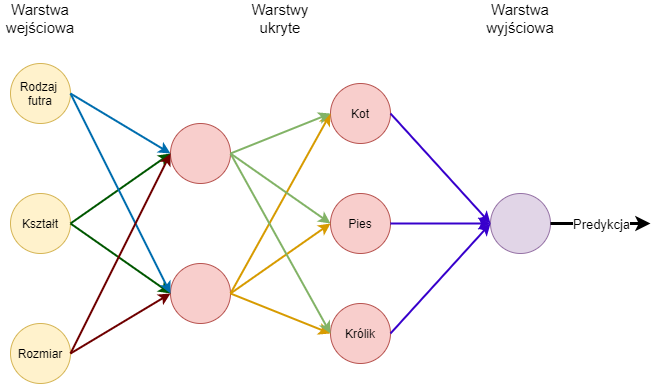
\includegraphics[width=0.8\textwidth]{./Img/MLP.png}
    \caption{Graficzne przedstawienie perceptronu wielowarstwowego Źródło: Własne}
\end{figure}

\subsection{Drzewa decyzyjne}

Algorytm Decision trees polega na stworzeniu drzewa decyzyjnego, w którym korzeń i węzły
są poszczególnymi cechami zbioru danych, a liście odpowiadają klasom, które tym danym 
należy przypisać. Ostatnim elementem są krawędzie, którymi reprezentuje się wartości cech. 
Kroki algorytmu są następujące:
\begin{enumerate}
    \item wybranie najlepszej cechy,
    \item dodanie gałęzi odpowiadających poszczególnym wartościom wybranej cechy,
    \item podział zbioru danych na podzbiory zgodnie z wartościami cechy,
    \item jeżeli wszystkie elementy podzbiorów należą do tej samej klasy 
    zakończenie gałęzi liściem, w przeciwnym wypadku powtórzenie kroków 
    od 1 do 4 dla każdego podzbioru.
\end{enumerate}
Aby dokonać optymalnego podziału algorytm musi wybrać cechy powodujące jak najlepsze
podzielenie różnych klas, a więc niosące ze sobą największą ilość informacji.
Wykorzystuje się w tym celu entropię, której wartość pozwala określić średnią ilość 
informacji niesioną przez poszczególne cechy~\cite{MLAlgorithms}.
\begin{equation}
    H(x)=-\sum_{i=1}^n p(x_i) \log_2 p(x_i).
    \label{eq-entropy}
\end{equation}
Wzór na entropię ~\ref{eq-entropy}, gdzie \textit{p(x\textsubscript{i})} jest prawdopodobieństwem
wybrania klasy \textit{x\textsubscript{i}}
\begin{table}[h]
    \begin{tabularx}{\linewidth}{>{\parskip1ex}X@{\kern4\tabcolsep}>{\parskip1ex}X}
    \toprule
    \hfil\bfseries Zalety
    &
    \hfil\bfseries Wady
    \\\cmidrule(r{3\tabcolsep}){1-1}\cmidrule(l{-\tabcolsep}){2-2}
    
    %% PROS, seperated by empty line or \par
    łatwe do zinterpretowania wyniki oraz wygodne do zwizualizowania,\par
    automatyczna selekcja ważnych cech,\par 
    obecność cech zbędnych nie ma wpływu na poprawność,\par
    szybkie wykonywanie predykcji.\par
    &
    
    %% CONS, seperated by empty line or \par
    wrażliwy na przeuczenie,\par
    potrzeba stworzenia nowego drzewa podczas dodawania nowych danych,\par
    małe zmiany w danych treningowych maja duży wpływ na predykcję.\par
    
    \\\bottomrule
    \end{tabularx}
    \caption{Wady i zalety Drzew decyzyjnych}
\end{table}

\begin{figure}[h]
    \centering
    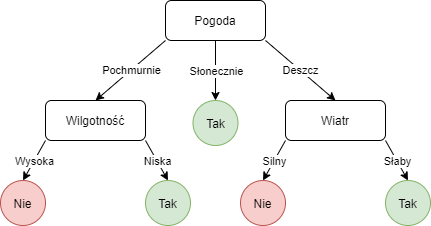
\includegraphics[width=0.8\textwidth]{./Img/BinaryTree.png}
    \caption{Przykładowe drzewo decyzyjne podejmujące decyzję czy wyjść na zewnątrz Źródło: Własne}
\end{figure}

\subsection{Las losowy}
Algorytm lasów losowych (Random forest) w skrócie RF, polega na stworzeniu lasu składającego się z drzew decyzjnych, 
które są budowane w następujący sposób:
\begin{itemize}
    \item z danych treningowych wybrane zostają losowe obiekty (może nastąpić wybranie tego samego obiektu dwukrotnie),
    \item wybrane obiekty stają się nowym zbiorem treningowym,
    \item w nowym zbiorze wybrana zostaje określona liczba losowych cech,
    \item tworzone zostaje drzewo decyzjne oparte tylko i wyłącznie na wybranych wcześniej cechach
    \item poprzednie kroki są powtarzane do czasu stworzenia określonej liczby drzew zazwyczaj jest to 
    liczba między 64 a 128 drzewami. 
\end{itemize}
Po stworzeniu wielu drzew decyzyjnych model jest gotowy aby wykonywać predykcje.
Predykcja w algorytmie RF jest wykonywana na podstawie głosowania przez każde stworzone drzewo na klasy. W głosowaniu 
tym wybrana zostaje klasa, na którą głosowała większość drzew ~\cite{randomforest}.

\begin{table}[H]
    \begin{tabularx}{\linewidth}{>{\parskip1ex}X@{\kern4\tabcolsep}>{\parskip1ex}X}
    \toprule
    \hfil\bfseries Zalety
    &
    \hfil\bfseries Wady
    \\\cmidrule(r{3\tabcolsep}){1-1}\cmidrule(l{-\tabcolsep}){2-2}
    
    %% PROS, seperated by empty line or \par
    odporny na overfitting,\par
    pojawienie się nowych danych nie wymaga tworzenia modelu od nowa,\par
    zachowuje poprawność w przypadku brakujących danych.\par
    
    &
    
    %% CONS, seperated by empty line or \par
    ciężkie do zinterpretowania wyniki z powodu ilości drzew,\par
    długi czas uczenia,\par
    nie sprawdza się dobrze w przypadku problemów regresyjnych\par
    
    \\\bottomrule
    \end{tabularx}
    \caption{Wady i zalety RF}
\end{table}

\subsection{Naiwny klasyfikator Bayesowski}

Naiwny klasyfikator Bayesowski (Naive Bayes) jest probabilistycznym klasyfikatorem, który
zakłada wzajemną niezależność wszystkich cech, stąd naiwność algorytmu. Stworzony przez niego model
opiera się na obliczeniu prawdopodobieństw wystąpienia poszczególnych cech pod warunkiem, że 
występują one w danej klasie. Pozwala to przy użyciu twierdzenia Bayesa ~\ref{eq:bayes} obliczyć prawdopodobieństwa 
warunkowe, określające z jak dużą pewnością występująca kombinacja cech prowadzi do 
wystąpienia różnych klas, na podstawie czego algorytm wykonuje predykcję~\cite{MLAlgorithms}. 


\begin{equation}
    \label{eq:bayes}
    P(A|B) = \frac{P(A|B)P(A)}{P(B)}
\end{equation}
gdzie P(A) i P(B) prawdopodobieństwa wystąpienia zdarzeń A i B, P(A|B) prawdopodobieństwo wystąpienia
zdarzenia A pod warunkiem wystąpienia zdarzenia B.

Algorytm ten jest często wykorzystywany w systemach czasu rzeczywistego, ponieważ działa bardzo szybko jednak
jego poprawność w porównaniu do bardziej skomplikowanych algorytmów jest mniejsza.
\begin{table}[h]
    \begin{tabularx}{\linewidth}{>{\parskip1ex}X@{\kern4\tabcolsep}>{\parskip1ex}X}
    \toprule
    \hfil\bfseries Zalety
    &
    \hfil\bfseries Wady
    \\\cmidrule(r{3\tabcolsep}){1-1}\cmidrule(l{-\tabcolsep}){2-2}
    
    %% PROS, seperated by empty line or \par
    bardzo szybki nawet w przypadku przewidywania wieloklasowego,\par
    działa nawet dla małej ilości danych,\par
    dobra poprawność w przypadku klasyfikacji danych wielowymiarowych
    jak na przykład w przypadku klasyfikacji tekstu.\par
    
    &
    
    %% CONS, seperated by empty line or \par
    jeżeli pewna cecha nie pojawi się w danych treningowych, a istnieje w danych 
    testowych algorytm nie będzie w stanie wykonać jego predykcji,\par
    przyjmuje niezależność cech co w rzeczywistości jest prawie niespotykane,\par
    mniejsza poprawność w porównaniu z bardziej skomplikowanymi algorytmami.\par
    
    \\\bottomrule
    \end{tabularx}
    \caption{Wady i zalety Naive Bayes}
\end{table}



\chapter{Przetwarzanie języków naturalnych}
Systemy przetwarzania języków naturalnych (\textbf{Natural language processing}) nazywane 
w skrócie NLP, oznaczają systemy mogące zrozumieć mowę i pismo ludzkie w takiej
formie jaką ludzie posługują się na co dzień. Programy takie mogą wykonywać zadania od zliczania
częstotliwości występowania danego słowa w tekście do automatycznego pisania artykułów. 

Głównym problemem w tworzeniu tego typu systemów jest to, że do komunikacji z komputerem zazwyczaj
potrzebne jest posługiwanie się precyzyjnymi komendami danego języka programowania, mowa ludzka
jednak nie zawsze jest precyzyjna i jej znaczenie może różnić się w zależności od kontekstu czy
różnego rodzaju regionalnych dialektów. Systemy NLP są często wykorzystywane w takich 
celach jak:
\begin{itemize}
    \item asystenci głosowi na przykład (\textit{Siri, Alexa, Cortana}) - są to urządzenia, które 
    wykonują komendy wypowiedziane w ich kierunku przez użytkownika,
    \item wyodrębnianie ważnych informacji z tekstu w celu późniejszej analizy,
    \item analiza sentymentu czyli wnioskowanie na podstawie tekstu opinii użytkowników na dany temat,
    \item sprawdzanie błędów ortograficznych,
    \item tłumaczenie tekstu na inne języki,
    \item chatboty wykorzystywane przez wiele firm w celu posiadania całodobowej zautomatyzowanej obsługi klienta.
\end{itemize}
Rozwój NLP ma bardzo duże znaczenie dla osób niepełnosprawnych, które często tylko dzięki ich pomocy są 
w stanie nawiązać interakcję z technologią pozwalającą im na znaczne podniesienie jakości życia. ~\cite{TextProcessing}
\section{Przygotowywanie danych tekstowych}
Aby ułatwić analizę ogromnej ilości danych tekstowych potrzebnych do poprawnego nauczenia systemu NLP,
wykonuje się na nich różnego rodzaju operacje. Operacje te powodują, że tekst nie traci swoich najważniejszych cech 
natomiast znacznie zmniejsza się moc obliczeniowa potrzebna do nauki algorytmów uczących wykonywanych na nim. 
Najczęściej wykorzystywanymi tego typu operacjami są ~\cite{preprocessing}:
\begin{itemize}
    \item zamiana wszystkich dużych liter na małe,
    \item usunięcie znaków specjalnych,
    \item usunięcie tak zwanych ``Stop words'' - są to bardzo często występujące w danym języku słowa, które 
    zazwyczaj nie wnoszą istotnych dla analizy informacji,
    \item tokenizacja - polega na podziale tekstu na mniejsze części zwane tokenami. W przypadku dużych bloków 
    tekstu może to być podział na zdania, a w przypadku zdań podział na słowa itd.,
    \item lematyzacja - oznacza ona sprowadzenie grupy wyrazów stanowiących odmianę danego zwrotu do wspólnej postaci,
    co pozwala na traktowanie ich jako to samo słowo,
    \item stemming - jest to proces usunięcia końcówki fleksyjnej pozostawiając tylko temat czyli nośnik znaczenia 
    wyrazu.
\end{itemize}
Wykonanie wybranych operacji na tekście daje na wyjściu skrócone dane tekstowe, które można następnie przeanalizować lub 
wykonać na nich wektoryzację, co pozwala na wykorzystanie ich w różnych algorytmach uczenia maszynowego. 
\section{Wektoryzacja}
Z uwagi na fakt, że algorytmy sztucznej inteligencji potrafią uczyć się tylko z danych przedstawionych w formie numerycznej, aby móc 
wykorzystać je w kombinacji z NLP potrzebny jest pewien sposób zamiany formy tekstowej na liczbową, tak by straciły one jak najmniej
swoich najważniejszych cech a zarazem były czytelne dla maszyny. 

Operacje takie nazywa się wektoryzacją tekstu, ponieważ 
reprezentacja liczbowa będąca ich wynikiem to najczęściej wektory. 
Wybór poprawnego sposobu zamiany tekstu może mieć ogromne znaczenie dla efektywności nauczonego modelu.

Jedne z najpopularniejszych metod wektoryzacji to: ~\cite{ML}
\begin{itemize}
    \item \textbf{Bag of words} jest to metoda wektoryzacji, w której każdemu unikalnemu symbolowi z tekstu przypisuje się liczbę 
    odpowiadającej jego ilości w analizowanym tekście. Symbolami mogą być całe zdania, słowa bądź NGramy. 
    Metoda ta w żaden sposób nie zachowuje informacji o porządku ani kontekście występujących symboli a jedynie o 
    częstotliwości ich występowania. 
    
    Wektor wynikowy metody ``Bag of words'' ma wymiar równy liczbie unikalnych symboli w tekście, przez co przy analizie dużej ilości 
    dokumentów ma dużą złożoność pamięciową aby naprawić ten problem najpierw na danych wykonuje się metody przygotowywania danych tekstowych.

    \item \textbf{TFIDF} (ang. Term frequency inverse document frequency) jest to metoda przypisująca, każdemu symbolowi 
    jego wagę w kontekście analizowanych dokumentów. Aby obliczyć tę wagę potrzebne są dwa elementy:
    \begin{enumerate}
        \item częstość symboli - którą uzyskuje się dzieląc liczbę wystąpień symbolu przez liczbę symboli w całym dokumencie,
        \item odwrotną częstość w dokumentach.
    \end{enumerate}
    Po obliczeniu obu tych wartości oblicza się tzw. TFIDF score, której wartość określa jak ważny jest dany symbol 
    dla dokumentu w kontekście wykonywanej analizy. Wynik ten oblicza się na podstawie wzoru \ref{eq:tfidf}, gdzie
    \begin{itemize}
        \item x - symbol,
        \item y - dokument,
        \item TF - częstość symbolu,
        \item N - ilość wszystkich dokumentów,
        \item df - ilość dokumentów w których pojawił się symbol x.
    \end{itemize}

    \begin{equation}
        \label{eq:tfidf}
        TFIDF_x,_y = TF_x,_y* \log{\frac{N}{df_x}}
    \end{equation}
\end{itemize}
\chapter{Projekt i implementacja systemu}
Do wykonania badań efektywności algorytmów uczenia maszynowego w rozpoznawaniu
fałszywych informacji potrzebne było stworzenie systemu, który w prosty sposób 
dla każdego z badanych algorytmów wykonałby operację uczenia go na danych treningowych,
a następnie sprawdził jak dobrze przewiduje on przypadki ze zbioru testowego.
System musi w odpowiedni sposób przygotować dane tekstowe przy użyciu metod takich jak zamiana dużych liter na małe, usuwanie znaków interpunkcyjnych itd.
Ważną funkcjonalnością oprogramowania jest też to by dzielił on dane tekstowe na 
różnej długości ngramy. 

ngramy są to sekwencje następujących po sobie jednostek, którymi mogą być słowa, 
głoski lub litery. W pracy wykonane zostaną badania różnych algorytmów klasyfikacji
na podstawie podziału na różnej długości literowe ngramy, a następnie wyniki zostaną
porównane w celu odnalezienia optymalnych ustawień do rozpoznawania Fake newsów.

System pozwoli na zbadanienwyników algorytmów takich jak poprawność predykcji oraz 
czasy trwania poszczególnych faz.

\section{Wykorzystane technologie}
Najpopularniejszymi językami programowania wykorzystywanymi do tworzenia modeli uczenia
maszynowego są:
\begin{itemize}
    \item Python,
    \item R,
    \item Lisp,
    \item Prolog.
\end{itemize}
Do wykonania systemu został wybrany język Python w wersji 3.8.5, jest to interpretowalny
język wysokiego poziomu powstały w roku 1991. Został on wybrany 
ponieważ posiada dużą ilość bibliotek takich jak: 
\begin{itemize}
    \item Scikit-learn,
    \item PySpark,
    \item PyTorch,
    \item TensorFlow,
    \item Keras.
\end{itemize}
Biblioteki te znacznie ułatwiają korzystanie z możliwości uczenia maszynowego.
W pracy zostanie wykorzystana biblioteka scikit-learn w wersji 0.23, która zawiera wszystkie 
testowane algorytmy i pozwala na bardzo wygodną ich implementację. Posiada także obie 
badane metody wektoryzacji tekstu, czyli Bag of words oraz TFIDF. Jest ona udostępniana na zasadach licencji BSD ~\cite{scikitlearn}. 
Licencja ta pozwala na użytkowanie i redystrybucję kodu zarówno zmodyfikowanego, jak i oryginalnego.

Ostatnią biblioteką potrzebną do stworzenia systemu była Natural Language Toolkit nazywana w skrócie 
NLTK. Jest to biblioteka służąca do przetwarzania języków naturalnych, która pozwala na proste przygotowanie tekstu do jego analizy
\section{Wymagania funkcjonalne}
Aplikacja powinna spełniać następujące wymagania funkcjonalne: 
\begin{itemize}
    \item wczytywać dane z zewnętrznego pliku w formacie csv,
    \item w odpowiedni sposób przygotowywać dane,
    \item dzielić dane na treningowe oraz testowe,
    \item wykonywać uczenie badanych algorytmów na danych treningowych,
    \item testować nauczone modele na danych testowych,
    \item zapisywać wyniki badań do pliku w formacie csv.
\end{itemize}
Są to funkcjonalności kluczowe aby system pozwalał wykonywać ważne dla osiągnięcia celu
badania. 
\section{Implementacja}
Implementacja składa się z dwóch funkcji służących do przygotowywania danych tekstowych
do późniejszej analizy oraz jednej pętli głównej, która wykonuje wszystkie badania,
a następnie zapisuje je do pliku w formacie csv. 

W systemie tworzony jest także obiekt
wielowymiarowej mapy, który po zakończeniu wykonywania programu przechowuje
wszystkie nauczone modele wektoryzacji oraz uczenia maszynowego. Zapisanie go za pomocą
biblioteki takiej jak \textit{Pickle} pozwala
w prosty sposób użyć i przetestować modele na dowolnych danych testowych. 


\begin{lstlisting}[language=Python, caption={Funkcja przygotowywująca dane pobrane z pliku csv}, captionpos=b, frame=single]
def basicPreparation(fileName): 
    file = pd.read_csv(fileName)
    label_encoder = preprocessing.LabelEncoder()
    file['label'] = label_encoder.fit_transform
        (file['label']) 
    file = file.applymap
        (lambda s: s.lower() if type(s) == str else s) 
    return (file['text'], file['label'])
\end{lstlisting}
Pierwsza funkcja \textit{basicPreparation} przyjmuje tylko jeden argument, którym jest
nazwa pliku. Metoda ta wczytuje do pamięci dane z pliku csv a następnie wykorzystuje
tzw. LabelEncoder, który pozwala na wykonanie zamiany etykiet w zbiorze danych na formę
numeryczną, w tym przypadku zamienia ona wartości REAL i FAKE na 0 i 1. Ostatnią 
akcją wykonywaną przez funkcję jest zamiana wszystkich liter zawartych w danych na małe.

Funkcja ta zwraca krotkę zawierającą dwa elementy:
\begin{itemize}
    \item listę artykułów,
    \item listę etykiet.
\end{itemize} 

\begin{lstlisting}[language=Python, caption={Funkcja przygotowywująca dane tekstowe}, captionpos=b, frame=single]
def dataPreprocessing(articles, labels):
    deletionIndexes = []
    for articleIndex in range(len(articles)):
        articles[articleIndex] = 
            ''.join(w+' ' for w in articles[articleIndex]
            .split(' ') if not w in stop_words and w != '')  
        articles[articleIndex] = 
            re.sub(r'[^a-zA-Z]+', ' ', articles[articleIndex])
        articleLength = len(articles[articleIndex])
        if(articleLength == 0 
            or articleLength < 500 
            or articleLength > 5000):
            deletionIndexes.append(articleIndex) 
    articles = articles.drop(deletionIndexes, axis=0)
    labels = labels.drop(deletionIndexes, axis=0)
    return (articles, labels)

\end{lstlisting}

Drugą funkcją znajdującą się w programie jest \textit{dataPreprocessing}. Posiada 
ona dwa argumenty:
\begin{itemize}
    \item articles - lista artykułów,
    \item labels - lista etykiet.
\end{itemize}
Funkcja ta wykonuje przygotowanie tekstu do późniejszej wektoryzacji. Wykonuje ona 
kolejno operacje:
\begin{itemize}
    \item usunięcia Stop words z tekstu każdego artykułu,
    \item usunięcia wszystkich znaków nie będących literami,
    \item usunięcia ze zbioru danych artykułów o długości poniżej 500 znaków oraz powyżej 5000 znaków,
    ponieważ przekazują one niepotrzebną ilość informacji.
\end{itemize}
Funkcja ta zwraca dokładnie taką samą krotkę jak \textit{basicPreparation}.


Główna pętla programu wykonuje kolejno następujące operacje:
\begin{itemize}
    \item wytrenowanie modelu wektoryzatora na danych treningowych,
    \item wektoryzacja danych treningowych i testowych za pomocą 
    nauczonego wcześniej modelu,
    \item normalizacja cech za pomocą StandardScaler,
    \item trening algorytmu na cechach treningowych funkcją \textit{fit},
    \item obliczenie efektywności funkcją \textit{score} na danych testowych,
    \item zapisanie wyników do pliku csv o tytule odpowiadającym nazwie algorytmu 
    uczenia maszynowego.
\end{itemize}
Aby obliczyć czas trwania faz uczenia i predykcji wykorzystano bibliotekę time w celu
zapisania czasu przed i po wykonaniu każdej z faz, a następnie odjęciu od siebie tych wartości.
\chapter{Ocena eksperymentalna}

\section{Cel Badań}
Celem badań jest sprawdzenie jak zmiana długości Ngramów podczas ekstrakcji cech
z tekstu wpływa na możliwości predykcyjne jednych z najpopularniejszych algorytmów 
uczenia maszynowego. 
\section{Warunki przeprowadzonego eksperymentu}

\section{Wyniki}

\begin{table}[h!]
    \centering
    \begin{tabular}{ | l | c | c | c | c | c | c | c | c |}
        \hline
        Rozmiar Ngramu & 1 & 2 & 3 & 4 & 5 & 6 & 7 & 8  \\ \hline
        Efektywność & 23\% & 23\% & 23\% & 23\% & 23\% & 23\% & 23\% & 23\%   \\ \hline
        Czas fazy uczenia & 23\% & 23\% & 23\% & 23\% & 23\% & 23\% & 23\% & 23\%  \\ \hline
    \end{tabular}
    \caption{Wyniki algorytmu KNN wektoryzacja metodą Bag of words}
\end{table}

\begin{table}[h!]
    \centering
    \begin{tabular}{ | l | c | c | c | c | c | c | c | c |}
        \hline
        Rozmiar Ngramu & 1 & 2 & 3 & 4 & 5 & 6 & 7 & 8  \\ \hline
        Efektywność & 23\% & 23\% & 23\% & 23\% & 23\% & 23\% & 23\% & 23\%   \\ \hline
        Czas fazy uczenia & 23\% & 23\% & 23\% & 23\% & 23\% & 23\% & 23\% & 23\%  \\ \hline
    \end{tabular}
    \caption{Wyniki algorytmu KNN wektoryzacja metodą TFIDF}
\end{table}

\begin{table}[h!]
    \centering
    \begin{tabular}{ | l | c | c | c | c | c | c | c | c |}
        \hline
        Rozmiar Ngramu & 1 & 2 & 3 & 4 & 5 & 6 & 7 & 8  \\ \hline
        Efektywność & 23\% & 23\% & 23\% & 23\% & 23\% & 23\% & 23\% & 23\%   \\ \hline
        Czas fazy uczenia & 23\% & 23\% & 23\% & 23\% & 23\% & 23\% & 23\% & 23\%  \\ \hline
    \end{tabular}
    \caption{Wyniki algorytmu SVC wektoryzacja metodą Bag of words}
\end{table}

\begin{table}[h!]
    \centering
    \begin{tabular}{ | l | c | c | c | c | c | c | c | c |}
        \hline
        Rozmiar Ngramu & 1 & 2 & 3 & 4 & 5 & 6 & 7 & 8  \\ \hline
        Efektywność & 23\% & 23\% & 23\% & 23\% & 23\% & 23\% & 23\% & 23\%   \\ \hline
        Czas fazy uczenia & 23\% & 23\% & 23\% & 23\% & 23\% & 23\% & 23\% & 23\%  \\ \hline
    \end{tabular}
    \caption{Wyniki algorytmu SVC wektoryzacja metodą TFIDF}
\end{table}

\begin{table}[h!]
    \centering
    \begin{tabular}{ | l | c | c | c | c | c | c | c | c |}
        \hline
        Rozmiar Ngramu & 1 & 2 & 3 & 4 & 5 & 6 & 7 & 8  \\ \hline
        Efektywność & 23\% & 23\% & 23\% & 23\% & 23\% & 23\% & 23\% & 23\%   \\ \hline
        Czas fazy uczenia & 23\% & 23\% & 23\% & 23\% & 23\% & 23\% & 23\% & 23\%  \\ \hline
    \end{tabular}
    \caption{Wyniki algorytmu Naive Bayes wektoryzacja metodą Bag of words}
\end{table}

\begin{table}[h!]
    \centering
    \begin{tabular}{ | l | c | c | c | c | c | c | c | c |}
        \hline
        Rozmiar Ngramu & 1 & 2 & 3 & 4 & 5 & 6 & 7 & 8  \\ \hline
        Efektywność & 23\% & 23\% & 23\% & 23\% & 23\% & 23\% & 23\% & 23\%   \\ \hline
        Czas fazy uczenia & 23\% & 23\% & 23\% & 23\% & 23\% & 23\% & 23\% & 23\%  \\ \hline
    \end{tabular}
    \caption{Wyniki algorytmu Naive Bayes wektoryzacja metodą TFIDF}
\end{table}

\begin{table}[h!]
    \centering
    \begin{tabular}{ | l | c | c | c | c | c | c | c | c |}
        \hline
        Rozmiar Ngramu & 1 & 2 & 3 & 4 & 5 & 6 & 7 & 8  \\ \hline
        Efektywność & 23\% & 23\% & 23\% & 23\% & 23\% & 23\% & 23\% & 23\%   \\ \hline
        Czas fazy uczenia & 23\% & 23\% & 23\% & 23\% & 23\% & 23\% & 23\% & 23\%  \\ \hline
    \end{tabular}
    \caption{Wyniki algorytmu Random Forest wektoryzacja metodą Bag of words}
\end{table}

\begin{table}[h!]
    \centering
    \begin{tabular}{ | l | c | c | c | c | c | c | c | c |}
        \hline
        Rozmiar Ngramu & 1 & 2 & 3 & 4 & 5 & 6 & 7 & 8  \\ \hline
        Efektywność & 23\% & 23\% & 23\% & 23\% & 23\% & 23\% & 23\% & 23\%   \\ \hline
        Czas fazy uczenia & 23\% & 23\% & 23\% & 23\% & 23\% & 23\% & 23\% & 23\%  \\ \hline
    \end{tabular}
    \caption{Wyniki algorytmu Random Forest wektoryzacja metodą TFIDF}
\end{table}

\begin{table}[h!]
    \centering
    \begin{tabular}{ | l | c | c | c | c | c | c | c | c |}
        \hline
        Rozmiar Ngramu & 1 & 2 & 3 & 4 & 5 & 6 & 7 & 8  \\ \hline
        Efektywność & 23\% & 23\% & 23\% & 23\% & 23\% & 23\% & 23\% & 23\%   \\ \hline
        Czas fazy uczenia & 23\% & 23\% & 23\% & 23\% & 23\% & 23\% & 23\% & 23\%  \\ \hline
    \end{tabular}
    \caption{Wyniki algorytmu MLP wektoryzacja metodą Bag of words}
\end{table}

\begin{table}[h!]
    \centering
    \begin{tabular}{ | l | c | c | c | c | c | c | c | c |}
        \hline
        Rozmiar Ngramu & 1 & 2 & 3 & 4 & 5 & 6 & 7 & 8  \\ \hline
        Efektywność & 23\% & 23\% & 23\% & 23\% & 23\% & 23\% & 23\% & 23\%   \\ \hline
        Czas fazy uczenia & 23\% & 23\% & 23\% & 23\% & 23\% & 23\% & 23\% & 23\%  \\ \hline
    \end{tabular}
    \caption{Wyniki algorytmu MLP wektoryzacja metodą TFIDF}
\end{table}
\section{Analiza wyników wraz z oceną statystyczną}

\section{Wnioski z badań}


\chapter{Podsumowanie}
Celem pracy było sprawdzenie czy algorytmy uczenia maszynowego mogą zostać wykorzystane
w detekcji tak zwanych \textit{fake newsów} i jak dobrze wykonają to zadanie. Cel pracy został osiągnięty,
a otrzymane wyniki jednoznacznie wskazują, że tego typu algorytmy bez większych problemów dobrze 
radzą sobie z klasyfikacją nieprawdziwych informacji.


W baniach postanowiono sprawdzić metodę podziału tekstu na rożnej długości ngramy i zwrócić uwagę 
jak zmiana ich długości wpływa na poszczególne cechy algorytmów.
Wyniki badań wykonanych na algorytmach: \textit{k}-NN, RF, Naive Bayes,
SVC oraz MLP pokazują, że algorytmy uczenia z całą pewnością mogą znaleźć swoje miejsce w systemach
automatycznego rozpoznawania fałszywych informacji. Wiele z nich nie miało problemu z osiągnięciem 
efektywności powyżej 90\%. Najlepszym z badanych algorytmów okazał się RF osiągając
wynik 99.82\%. Najgorzej z zadaniem poradziła sobie metoda \textit{k}-NN, jej najwyższa 
poprawność wynosiła 80.07\%.

Jak przypuszczano, ogromne znaczenie dla efektywności
miała zmiana długości ngramów, które nie mogą być ani za krótkie, ani za długie.
Dla wszystkich badanych algorytmów za wyjątkiem \textit{k}-NN, ngramy o długości 1 dały najgorsze wyniki, a wartości
pośrednie najlepsze.

Istotnym problemem z tego typu rozwiązaniami jest brak zbiorów treningowych posiadających 
artykuły o zróżnicowanej tematyce. Większość istniejących danych zawiera głównie artykuły związane z 
polityką, z uwagi na to właśnie z taką tematyką algorytmy poradziłyby sobie najlepiej. Mogłyby mieć one jednak problem 
z artykułami naukowymi, sportowymi itp.

Jednym ze sposobów na dalszy rozwój pracy mogłoby być opracowanie systemu rozpoznającego 
przerobione obrazy. System taki w kombinacji z wykrywaniem fałszywych tekstów zawartym
w niniejszej pracy jeszcze bardziej zwiększyłby poprawność detekcji \textit{fake newsów} i stanowiłby 
duży krok w wyeliminowaniu z internetu zagrożenia jakim są nieprawdziwe informacje.

%\bibliographystyle{plalpha}
\bibliographystyle{plabbrv}

%UWAGA: bibliotekę referencji należy przygotować samemu. Dobrym do tego narzędziem jest JabRef.
%       Nazwę przygotowanej biblioteki wpisuje się poniżej bez rozszerzenia 
%       (w tym przypadku jest to "dokumentacja.bib")
\bibliography{dokumentacja}
\appendix
\chapter{Opis załączonej płyty CD/DVD}
Na załączonej płycie znajduje się niniejsza praca w formacie PDF oraz pliki z kodem źródłowym
aplikacji wykorzystanej do wykonania badań. 

\chapterstyle{noNumbered}
\phantomsection % sets an anchor
\addcontentsline{toc}{chapter}{Indeks rzeczowy}
\printindex

\end{document}
